\documentclass[12pt]{amsart}
\usepackage{amssymb}
\usepackage{amsmath}
\usepackage{latexsym}
\usepackage{tikz}
\usepackage{hyperref}
\hypersetup{colorlinks=true,citecolor=blue,linkcolor=blue}


% add yourself here in order to make comments on the side
\usepackage[draft]{say}
\newcommand{\saySS}[1]{\say[SS]{#1}}
\newcommand{\sayMC}[1]{\say[MC]{#1}}
\newcommand{\sayMG}[1]{\say[MG]{#1}}

% ambients
\newtheorem{lemma}{Lemma}[section]
\newtheorem{theorem}{Theorem}[section]
\newtheorem{propo}[theorem]{Proposition}
\newtheorem{prop}[theorem]{Proposition}
\newtheorem{cor}[theorem]{Corollary}
\newtheorem{conj}[theorem]{Conjecture}
\newtheorem{claim}[theorem]{Claim}
\newtheorem{claim*}{Claim}
\newtheorem{rmk}[theorem]{Remark}
\newtheorem{thm}[theorem]{Theorem}
\newtheorem{defn}[theorem]{Definition}
\theoremstyle{remark}
\newtheorem{example}[theorem]{Example}
\newtheorem{remark}[theorem]{Remark}
\newtheorem{question}[theorem]{Question}
\numberwithin{equation}{section}

% shorthands
\newcommand{\QQ}{\mathbb{Q}}
\newcommand{\ZZ}{\mathbb{Z}}
\newcommand{\NN}{\mathbb{N}}
\newcommand{\RR}{\mathbb{R}}
\newcommand{\cA}{\mathcal{A}}
\newcommand{\Hom}{\operatorname{Hom}}
\newcommand{\dd}{\mathfrak{d}}
\newcommand{\fod}{\mathfrak{d}}
\newcommand{\DD}{\mathfrak{D}}
\newcommand{\fom}{\mathfrak{m}}
\newcommand{\gr}{\mathrm{gr}}
\newcommand{\Mono}{\operatorname{Mono}}
\newcommand{\Spec}{\operatorname{Spec}}

%%%%%%%%%%%%%%%%%%%%%%%%%%%%%%%%%%%%%%%%%%%%%%%%%%%%%%%%%%%%%%%%%%%
\title{Theta functions and greedy bases}
\author{CCGMMRSW}

\begin{document}
\maketitle

\section{Scattering diagrams and broken lines}
\saySS{We are using Fock-Goncharov conventions through the paper; in particular
  we denote initial cluster variables by $A_i$ and we read mutations by rows.
  All the relevant notions, (in particular $d$- and $g$-vectors) are
  the ``transposed'' of those in Fomin-Zelevinsky and Lee-Li-Zelevinsky. We
  should mention these facts in the introduction.}
In this section, we will describe the cluster algebras $\cA (b,c)$ from the
point of view of scattering diagrams. While all the results in this section are
derived from \cite{GHKK}, we will adopt a slightly simplified notation here
sufficient for the rank $2$ case.

Let $N = \ZZ^2$ be a lattice and $M = \Hom (N, \ZZ)$. Write $M_{\RR} = M \otimes
\RR$, $N_{\RR} = N\otimes \RR$. Take $\Bbbk$ to be a field of characteristic 0.
Fix a basis $f_1, f_2$ of $M$, and let $A_1,A_2$ be the corresponding generators
of $\Bbbk[M]$. When convenient, given $m=a_1f_1+a_2f_2\in M$,  we will use the 
shorthand $z^m$ for the monomial $A_1^{a_1} A_2^{a_2}$.

Let $\sigma \subsetneq M_{\RR}$ be a strictly convex rational cone; set
$P=\sigma \cap M$, and write $\widehat{\Bbbk[P]}$ for the completion of the
monoid ring $\Bbbk[P]$ at the maximal monomial ideal $\fom$ generated by
$\left\{z^m \,|\, m\in P\setminus\{0\}\right\}$.

\begin{defn}
  \label{walldef}
  A \emph{wall} is a pair $(\dd, f_{\dd})$, where 
  \begin{itemize}

    \item 
      $\dd \subset M_{\mathbb{R}}$ is either a ray $\RR_{\le 0} m_0$ or a line
      $\RR m_0$ with $m_0\in \sigma \cap(M\setminus 0)$;

    \item 
      $f_{\dd} \in \widehat{\Bbbk [P]}$ is such that 
      \[ 
        f_{\dd} = f_{\dd}(z^{m_0}) = 1 + \sum_{k\geq 1} c_k z^{k m_0},
      \] 
      for some $c_k \in \Bbbk$. 
  \end{itemize}
  The set $\dd \subset M_{\mathbb{R}}$ is called the \emph{support} of the wall
  $(\dd, f_{\dd})$.
\end{defn}

\begin{defn}
  \label{def:scattering_diagram}
  A scattering diagram $\DD$ is a collection of walls such that, for each $k \geq
  0$, the set
  \[
    \{ (\dd, f_{\dd}) \in \DD\, |\, f_{\dd} \neq 1 \bmod \fom^k \}
  \]
  is finite. For semplicity we diverge slightly form the convention in
  \cite{GHKK} by requiring that $\dd_1 \neq \dd_2$ whenever $f_{\dd_1}\neq
  f_{\dd_2}$.
\end{defn}

For a scattering diagram $\DD$, we denote the support of $\DD$ as
\[
  \text{Supp} (\DD) := \bigcup_{(\dd, f_{\dd}) \in \DD} \dd. 
\]

To each wall $(\dd, f_{\dd})$, given a direction $v$ transversal to $\dd$, one
can associate the element $\theta_{v,\dd}\in
{\mathrm{Aut}}_{\Bbbk-alg}\big(\widehat{\Bbbk[P]}\big)$ defined by
\[
  \theta_{v,\dd} (z^m) := z^m f_{\dd}^{\langle m, n \rangle }, 
\]
where $n\in N$ is primitive, annihilates the tangent space to $\dd$, and is
uniquely determined by the sign convention $ \langle n, v \rangle <0$.  Note
that the only role of the transversal direction $v$ is to fix which of the two
normals $\pm n$ is used in the exponent. 

Consider a smooth immersion
\[  
  \gamma: [0,1] \rightarrow M_{\mathbb{R}} \backslash  \{0 \}  
\]
with endpoints not in the support of $\DD$. Assume $\gamma$ is transversal to
each wall of $\DD$ that it crosses. For each power $k \geq 1$, let  
\[
  0< t_1 <  t_2 < \cdots < t_s < 1 
\]
be the longest sequence of numbers such that $\gamma(t_i)\in\dd_i$ for some wall
$(\dd_i,f_{\dd_i}) \in \DD$ with $f_{\dd_i} \neq 1 \text{ mod } \fom^k$.

In view of the definition of scattering diagram, such a sequence is finite; we
can therefore consider the composition 
\[
  \theta^k_{\gamma, \DD} :=
  \theta_{\gamma'(t_s),\dd_s} \circ \cdots \circ \theta_{\gamma'(t_1),\dd_1}.
\]
Define the \textit{path-ordered product} along $\gamma$ as
\[
  \theta_{\gamma, \DD} := \lim_{k \rightarrow \infty} \theta ^k_{\gamma, \DD}. 
\]

\begin{defn}
  A scattering diagram is \emph{consistent} if $\theta _{\gamma, \DD}$ depends
  only on the endpoints of $\gamma$ for any path $\gamma$ for which
  $\theta_{\gamma, \DD}$ is well defined.
\end{defn}

\begin{theorem}[Kontsevich-Soibelman] 
  \label{KS}
  Given a scattering diagram $\DD$, there always exists a consistent scattering
  diagram $\DD'$ which contains $\DD$ such that $\DD'\setminus\DD$ only consists
  of rays.
\end{theorem}

We will now describe the scattering diagram $\DD_{(b,c)}$ associated to 
$\cA(b,c)$.
Recall that the initial exchange matrix in $\cA(b,c)$ is 
\[
  \epsilon = \begin{pmatrix} 0 & c\\ -b & 0\end{pmatrix},
\]
where $b$, $c$ are positive integers.  Following Example 1.30 of \cite{GHKK}, we
take $\sigma$ to be the second quadrant, i.e., the cone generated by $-f_1$ and
$f_2$. Then the ``initial'' scattering diagram associated to the above exchange
matrix is
\[
  \DD_{\mathrm{in},(b,c)} := 
  \big\{
    \big( \RR (-f_1), 1+A_1^{-b}\big), 
    \big( \RR f_2, 1+A_2^c\big) 
  \big\}.
\]

We will denote by $\DD_{(b,c)}$ the consistent scattering diagram obtained by
applying Theorem \ref{KS} to $\DD_{\mathrm{in},(b,c)}$.

\begin{example} 
  \label{ex}
  Consider $\cA(2,1)$. Then we get
  \[
    \DD_{\mathrm{in},(2,1)} =  
    \{ 
      (\RR (-f_1), 1+A_1^{-2}), 
      (\RR f_2, 1+A_2)  
    \}   
  \]
  and the associated consistent scattering diagram $\DD_{(2,1)}$ (shown in
  Figure~\ref{fig:diagex}) contains $\DD_{\mathrm{in},(2,1)}$ together with
  the two walls
  \[ 
    \left( \RR_{\leq 0} (-f_1+f_2), 1+A_1^{-2}A_2^2 \right)
    \quad \mbox{and} \quad
    \left( \RR_{\leq 0} (-2f_1+f_2), 1+A_1^{-2}A_2 \right).
  \]
\end{example}

\begin{figure}
  \centering
  \begin{tikzpicture}
    \draw (3,0) -- (-3,0) node[left] {$1+A_1^{-2}$};
    \draw (0,-3) -- (0,3) node[above] {$1+A_2$};
    \draw (0,0) -- (3,-3) node[below right] {$1+A_1^{-2}A_2^2$};
    \draw (0,0) -- (3,-1.5) node[below right] {$1+A_1^{-2}A_2$};
  \end{tikzpicture}
  \caption{The scattering diagram $\DD_{(2,1)}$} 
  \label{fig:diagex}
\end{figure}

For general $b$ and $c$, the diagram $\DD_{(b,c)} \backslash
\DD_{\mathrm{in},(b,c)}$ may consist of an infinite number of rays, and in fact
it is infinite precisely when $bc\ge 4$. A more detailed description of the rays
which appear can be found in \cite{GHKK}, Example 1.30. We summarize the crucial
points here.

First of all note that, in view of the definition of scattering diagram, all the
rays in  $\DD_{(b,c)} \backslash \DD_{\mathrm{in},(b,c)}$ are contained in the
fourth quadrant.  To make our next observation we need to extend the action of
linear operators on $M_\RR$ to an action on pairs $(\dd,f_\dd)$. If $S$ is
linear on $M_\RR$ set
\begin{equation}
  \label{eqn:linear action}
  S(\dd,f_\dd(z^{m_0}))
  :=
  \left( S(\dd), f_\dd(z^{S(m_0)}) \right)
\end{equation}
Note that, even if $(\dd,f_\dd)$ is a wall, $S(\dd,f_\dd)$ needs not be a wall
since $S(m_0)$ may lay outside of the cone $\sigma$ (in which case we also get
that  $f_\dd(z^{S(m_0)})$ is not an element of $\widehat{\Bbbk [P]}$).

Now consider the two linear involutions $S_1$ and $S_2$ given in the basis $f_1,
f_2$ by
\[
  S_1 =  
  \begin{pmatrix}
    -1 & -b \\
    0& 1
  \end{pmatrix}
  %
  \quad
  \mbox{and}
  \quad
  %
  S_2 =  
  \begin{pmatrix}
    1 & 0 \\
    -c & -1
  \end{pmatrix}.
\]
If $(\dd, f_{\dd}) \in \DD_{(b,c)} \backslash \DD_{\mathrm{in},(b,c)}$ and $S_i
(\dd)$ is contained strictly in the fourth quadrant, then $S_i(\dd, f_{\dd}) \in
\DD_{(b,c)} \backslash \DD_{\mathrm{in},(b,c)}$. Moreover both 
\begin{equation}
  \label{eq:first-walls}
  S_2(\RR_{\leq 0}(-f_1),1+A_1^{-b})
  %
  \quad
  \mbox{and}
  \quad
  %
  S_1(\RR_{\leq 0}(f_2),1+A_2^c)
\end{equation}
are walls in $\DD_{(b,c)} \backslash \DD_{\mathrm{in},(b,c)}$ (even though
neither 
\[
  (\RR_{\leq 0}(-f_1),1+A_1^{-b})
  %
  \quad
  \mbox{nor}
  \quad
  %
  (\RR_{\leq 0}(f_2),1+A_2^c)
\]
are walls in $\DD_{(b,c)}$). These considerations gives us a recipe to produce
elements of $\DD_{(b,c)} \backslash \DD_{\mathrm{in},(b,c)}$: it is enough to apply
alternatively $S_1$ and $S_2$ to the walls (\ref{eq:first-walls}).

We need to distinguish two cases. If $bc<4$ this procedure will construct, in
finitely many steps, all the walls in $\DD_{(b,c)} \backslash
\DD_{\mathrm{in},(b,c)}$.  If $bc\geq 4$, instead, we will get two infinite
families of walls whose supports will converge to the boundary of the convex cone
spanned by the irrational vectors
\[
  2bf_1+\left(-bc + \sqrt{bc(bc-4)}\right)f_2
  \quad
  \mbox{and}
  \quad
  2bf_1+\left(-bc - \sqrt{bc(bc-4)}\right)f_2
\]
These will exhaust all the walls in  $\DD_{(b,c)} \backslash \DD_{\mathrm{in},(b,c)}$
with support laying outside of this cone. The structure of the remaining part of 
$\DD_{(b,c)}$ is not completely understood; the expectation is that there is
a wall for each possible rational slope inside the irrational cone.
\sayMC{more detail at end?}
\sayMG{Wait and see what other facts we need about
  the diagram.} 

On the other hand the chamber structure one sees outside of the irrational cone
is very well-behaved and familiar in the theory of cluster algebras. This
chamber structure coincides with the Fock-Goncharov cluster complex, see
\cite{GHKK}, \S2, the mutation fan of Reading \cite{R}, and the picture group of
Igusa-Orr-Todorov-Weyman \cite{IOTW}.

\begin{figure}
  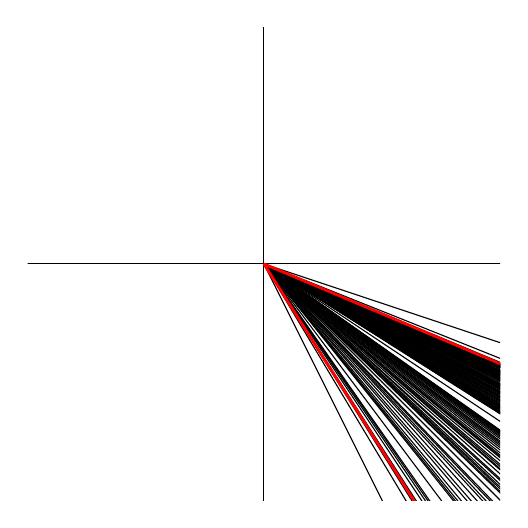
\begin{tikzpicture}[scale=0.1]
\clip (-30, -30) rectangle (30, 30);
\draw[color=black] (0,0) -- (-0.000000000000000, 60.0000000000000);
\draw[color=black] (0,0) -- (-60.0000000000000, -0.000000000000000);
\draw[color=black] (0,0) -- (-0.000000000000000, -60.0000000000000);
\draw[color=black] (0,0) -- (26.8328157299975, -53.6656314599950);
\draw[color=black] (0,0) -- (30.8697453256516, -51.4495755427527);
\draw[color=black] (0,0) -- (31.7999364001908, -50.8798982403053);
\draw[color=black] (0,0) -- (32.4454554788099, -50.4707085225932);
\draw[color=black] (0,0) -- (33.2820117735137, -49.9230176602706);
\draw[color=black] (0,0) -- (33.8002094784906, -49.5736405684529);
\draw[color=black] (0,0) -- (34.1525987298185, -49.3315314986267);
\draw[color=black] (0,0) -- (34.4077406617997, -49.1539152311424);
\draw[color=black] (0,0) -- (36.0000000000000, -48.0000000000000);
\draw[color=black] (0,0) -- (37.4817028532655, -46.8521285665818);
\draw[color=black] (0,0) -- (37.7002264252573, -46.6764708122233);
\draw[color=black] (0,0) -- (37.9942674154358, -46.4374379521993);
\draw[color=black] (0,0) -- (38.4110639798688, -46.0932767758426);
\draw[color=black] (0,0) -- (39.0474824073581, -45.5553961419178);
\draw[color=black] (0,0) -- (39.5102764721111, -45.1546016824127);
\draw[color=black] (0,0) -- (40.1378838973470, -44.5976487748300);
\draw[color=black] (0,0) -- (40.6968061639840, -44.0882066776493);
\draw[color=black] (0,0) -- (41.0364677328798, -43.7722322484051);
\draw[color=black] (0,0) -- (41.4285448009500, -43.4013326486143);
\draw[color=black] (0,0) -- (41.6481342350539, -43.1906577252411);
\draw[color=black] (0,0) -- (42.4264068711929, -42.4264068711929);
\draw[color=black] (0,0) -- (43.0740236070633, -41.7687501644250);
\draw[color=black] (0,0) -- (43.2192128094889, -41.6185012239522);
\draw[color=black] (0,0) -- (43.4482758620690, -41.3793103448276);
\draw[color=black] (0,0) -- (43.6207891529890, -41.1974119778230);
\draw[color=black] (0,0) -- (43.8633160945721, -40.9390950216007);
\draw[color=black] (0,0) -- (44.2292484120445, -40.5434777110408);
\draw[color=black] (0,0) -- (44.3964044037566, -40.3603676397788);
\draw[color=black] (0,0) -- (44.8445591210196, -39.8618303297952);
\draw[color=black] (0,0) -- (45.2263637944671, -39.4281120259456);
\draw[color=black] (0,0) -- (45.3413449673891, -39.2958323050705);
\draw[color=black] (0,0) -- (45.5553961419178, -39.0474824073581);
\draw[color=black] (0,0) -- (45.7505481223675, -38.8186468917058);
\draw[color=black] (0,0) -- (46.0932767758426, -38.4110639798688);
\draw[color=black] (0,0) -- (46.3844022289554, -38.0589967006814);
\draw[color=black] (0,0) -- (46.5140991310374, -37.9003770697341);
\draw[color=black] (0,0) -- (46.6346922424491, -37.7518937200779);
\draw[color=black] (0,0) -- (46.8521285665818, -37.4817028532655);
\draw[color=black] (0,0) -- (47.1295003336521, -37.1323335962108);
\draw[color=black] (0,0) -- (47.3611330425796, -36.8364368108952);
\draw[color=black] (0,0) -- (47.5574393462760, -36.5826456509815);
\draw[color=black] (0,0) -- (47.7259032019499, -36.3625929157714);
\draw[color=black] (0,0) -- (47.8720394353344, -36.1699853511415);
\draw[color=black] (0,0) -- (48.0000000000000, -36.0000000000000);
\draw[color=black] (0,0) -- (48.2134316006847, -35.7136530375442);
\draw[color=black] (0,0) -- (48.3842997513423, -35.4818198176510);
\draw[color=black] (0,0) -- (48.5241650581913, -35.2903018605028);
\draw[color=black] (0,0) -- (48.6407537039929, -35.1294332306615);
\draw[color=black] (0,0) -- (48.7394240154955, -34.9924069854839);
\draw[color=black] (0,0) -- (48.8240082724041, -34.8742916231458);
\draw[color=black] (0,0) -- (48.8973194741253, -34.7714271816002);
\draw[color=black] (0,0) -- (48.9614688660993, -34.6810404468203);
\draw[color=black] (0,0) -- (49.0180717958857, -34.6009918559193);
\draw[color=black] (0,0) -- (49.0683851580460, -34.5296043704768);
\draw[color=black] (0,0) -- (49.9230176602706, -33.2820117735137);
\draw[color=black] (0,0) -- (50.6527689148682, -32.1604881999163);
\draw[color=black] (0,0) -- (50.6891445332537, -32.1031248710607);
\draw[color=black] (0,0) -- (50.7293341818583, -32.0395794832789);
\draw[color=black] (0,0) -- (50.7739704053850, -31.9687961811684);
\draw[color=black] (0,0) -- (50.8238336704889, -31.8894642638361);
\draw[color=black] (0,0) -- (50.8798982403053, -31.7999364001908);
\draw[color=black] (0,0) -- (50.9433962264151, -31.6981132075472);
\draw[color=black] (0,0) -- (51.0159088012717, -31.5812768769777);
\draw[color=black] (0,0) -- (51.0994990022726, -31.4458455398601);
\draw[color=black] (0,0) -- (51.1969100191175, -31.2870005672385);
\draw[color=black] (0,0) -- (51.2519133368663, -31.1968168137447);
\draw[color=black] (0,0) -- (51.3118698932411, -31.0981029656007);
\draw[color=black] (0,0) -- (51.3774785130198, -30.9895902142024);
\draw[color=black] (0,0) -- (51.4495755427527, -30.8697453256516);
\draw[color=black] (0,0) -- (51.5291702980016, -30.7366980724922);
\draw[color=black] (0,0) -- (51.6174920180505, -30.5881434181040);
\draw[color=black] (0,0) -- (51.7160529094662, -30.4212075938036);
\draw[color=black] (0,0) -- (51.8267340539060, -30.2322615314452);
\draw[color=black] (0,0) -- (51.9084000879008, -30.0918261379135);
\draw[color=black] (0,0) -- (51.9519043946730, -30.0166558724777);
\draw[color=black] (0,0) -- (51.9973474124501, -29.9378666920167);
\draw[color=black] (0,0) -- (52.0945885274676, -29.7683363014100);
\draw[color=black] (0,0) -- (52.2013311509167, -29.5807543188528);
\draw[color=black] (0,0) -- (52.2587080645757, -29.4792712159145);
\draw[color=black] (0,0) -- (52.3190271231289, -29.3720854024583);
\draw[color=black] (0,0) -- (52.3503609569832, -29.3162021359106);
\draw[color=black] (0,0) -- (52.4494365672923, -29.1385758707179);
\draw[color=black] (0,0) -- (52.5568645648961, -28.9443601951602);
\draw[color=black] (0,0) -- (52.5947130467757, -28.8755287315631);
\draw[color=black] (0,0) -- (52.6257760704901, -28.8188773719351);
\draw[color=black] (0,0) -- (52.6737343748631, -28.7311278408344);
\draw[color=black] (0,0) -- (52.7234062015372, -28.6398749736745);
\draw[color=black] (0,0) -- (52.7575179922064, -28.5769889124452);
\draw[color=black] (0,0) -- (52.8013303601801, -28.4959560673988);
\draw[color=black] (0,0) -- (52.8282659953305, -28.4459893821010);
\draw[color=black] (0,0) -- (52.9411764705882, -28.2352941176471);
\draw[color=black] (0,0) -- (53.0420976185223, -28.0452470166899);
\draw[color=black] (0,0) -- (53.0630851708182, -28.0055171734874);
\draw[color=black] (0,0) -- (53.0950933429189, -27.9447859699573);
\draw[color=black] (0,0) -- (53.1498921168093, -27.8404196802335);
\draw[color=black] (0,0) -- (53.1950907699273, -27.7539604017012);
\draw[color=black] (0,0) -- (53.2652718869358, -27.6190298673000);
\draw[color=black] (0,0) -- (53.3172394232918, -27.5185751862151);
\draw[color=black] (0,0) -- (53.3384733855962, -27.4773953804586);
\draw[color=black] (0,0) -- (53.3890477687642, -27.3789988557765);
\draw[color=black] (0,0) -- (53.4260809317648, -27.3066635873465);
\draw[color=black] (0,0) -- (53.4543688141188, -27.2512468464135);
\draw[color=black] (0,0) -- (53.4947320855546, -27.1719274085357);
\draw[color=black] (0,0) -- (53.5221465618161, -27.1178875913202);
\draw[color=black] (0,0) -- (53.5419818370838, -27.0787034578355);
\draw[color=black] (0,0) -- (53.6656314599950, -26.8328157299975);
\draw[color=black] (0,0) -- (53.7807905522025, -26.6012512408744);
\draw[color=black] (0,0) -- (53.7978079632368, -26.5668187472774);
\draw[color=black] (0,0) -- (53.8207265847134, -26.5203580272501);
\draw[color=black] (0,0) -- (53.8532595862449, -26.4542327792080);
\draw[color=black] (0,0) -- (53.8752433636188, -26.4094330213818);
\draw[color=black] (0,0) -- (53.9030616551521, -26.3526079202966);
\draw[color=black] (0,0) -- (53.9393921302362, -26.2781653967817);
\draw[color=black] (0,0) -- (53.9888464317720, -26.1764103911622);
\draw[color=black] (0,0) -- (54.0330981818747, -26.0849439498705);
\draw[color=black] (0,0) -- (54.0601001855460, -26.0289371263740);
\draw[color=black] (0,0) -- (54.0913834480964, -25.9638640550863);
\draw[color=black] (0,0) -- (54.1089617234779, -25.9272108258332);
\draw[color=black] (0,0) -- (54.1716311294358, -25.7960148235409);
\draw[color=black] (0,0) -- (54.2361393319646, -25.6601089312521);
\draw[color=black] (0,0) -- (54.2549188047594, -25.6203783244697);
\draw[color=black] (0,0) -- (54.2891221320596, -25.5478221797928);
\draw[color=black] (0,0) -- (54.3194796673387, -25.4832126834428);
\draw[color=black] (0,0) -- (54.3334132954371, -25.4534909131777);
\draw[color=black] (0,0) -- (54.3709883997159, -25.3731279198674);
\draw[color=black] (0,0) -- (54.4130381386334, -25.2828258017893);
\draw[color=black] (0,0) -- (54.4312940646490, -25.2434986966488);
\draw[color=black] (0,0) -- (54.4480144271905, -25.2074140866623);
\draw[color=black] (0,0) -- (54.4775630700271, -25.1434906477048);
\draw[color=black] (0,0) -- (54.5141841179005, -25.0639926978853);
\draw[color=black] (0,0) -- (54.5438893736571, -24.9992826295928);
\draw[color=black] (0,0) -- (54.5684685351480, -24.9455856160677);
\draw[color=black] (0,0) -- (54.5891428975854, -24.9003107953898);
\draw[color=black] (0,0) -- (54.6219886477563, -24.8281766580710);
\draw[color=black] (0,0) -- (54.6469139903736, -24.7732676756360);
\draw[color=black] (0,0) -- (54.6664753703014, -24.7300721913268);
\draw[color=black] (0,0) -- (54.6822359795205, -24.6952033455899);
\draw[color=black] (0,0) -- (54.6952054133419, -24.6664651864091);
\draw[color=black] (0,0) -- (54.7060647954424, -24.6423715294786);
\draw[color=black] (0,0) -- (54.7152903105064, -24.6218806397279);
\draw[color=black] (0,0) -- (54.8286929172154, -24.3683079632069);
\draw[color=black] (0,0) -- (54.9311672413819, -24.1364219696981);
\draw[color=black] (0,0) -- (54.9386418114771, -24.1194037221119);
\draw[color=black] (0,0) -- (54.9472925276370, -24.0996897051039);
\draw[color=black] (0,0) -- (54.9574206857048, -24.0765843004040);
\draw[color=black] (0,0) -- (54.9694400941313, -24.0491300411825);
\draw[color=black] (0,0) -- (54.9839349968086, -24.0159716078015);
\draw[color=black] (0,0) -- (55.0017578825054, -23.9751252308357);
\draw[color=black] (0,0) -- (55.0242033751941, -23.9235666848670);
\draw[color=black] (0,0) -- (55.0377604843468, -23.8923611404916);
\draw[color=black] (0,0) -- (55.0533375185954, -23.8564462580580);
\draw[color=black] (0,0) -- (55.0714221576086, -23.8146690411280);
\draw[color=black] (0,0) -- (55.0926727722741, -23.7654666860790);
\draw[color=black] (0,0) -- (55.1180002415665, -23.7066667705663);
\draw[color=black] (0,0) -- (55.1275581099126, -23.6844323731477);
\draw[color=black] (0,0) -- (55.1487018010835, -23.6351579147501);
\draw[color=black] (0,0) -- (55.1730637090806, -23.5782323543079);
\draw[color=black] (0,0) -- (55.1866900848445, -23.5463211028670);
\draw[color=black] (0,0) -- (55.2014387393748, -23.5117239075115);
\draw[color=black] (0,0) -- (55.2092781377147, -23.4933098458360);
\draw[color=black] (0,0) -- (55.2349069125154, -23.4329908113702);
\draw[color=black] (0,0) -- (55.2642342869189, -23.3637413245511);
\draw[color=black] (0,0) -- (55.2749736846831, -23.3383222224218);
\draw[color=black] (0,0) -- (55.2981225082839, -23.2834200034880);
\draw[color=black] (0,0) -- (55.3846153846154, -23.0769230769231);
\draw[color=black] (0,0) -- (55.7086014531156, -22.2834405812462);
\draw[color=black] (0,0) -- (56.9209978830308, -18.9736659610103);
\draw[color=black] (0,0) -- (60.0000000000000, -0.000000000000000);
\draw[color=red, line width=1pt] (0,0) -- (60.0000000000000, -25.3589838486225);
\draw[color=red, line width=1pt] (0,0) -- (60.0000000000000, -94.6410161513775);

\end{tikzpicture}

  \caption{The supports of all the walls $(\dd,f_\dd)$ in $\DD_{(3,2)}$ such
    that $f_\dd \neq 1 \bmod \fom^{100}$; the boundary rays of
    the irrational cone are highlighted.} 
  \label{diagram32}
\end{figure}

The following result explains the connection between scattering diagrams
and the corresponding cluster algebras: 
\saySS{Wen we write the introductory part on cluster algebras we might want to
  mention what universal Laurent polynomials are}
\begin{theorem} 
  \label{univLaurent} 
  Let $\DD:=\DD_{(b,c)}$ as constructed above.  Let $f \in \Bbbk[M]$ be a
  Laurent polynomial. For any path $\gamma$ for which $\theta_{\gamma,\DD}$ is
  defined, $\theta_{\gamma,\DD}(f)$ can be viewed as an element of
  $\Bbbk[[A_1,A_2^{-1}]]$ localized at $A_1A_2^{-1}$. Then $f$ is a universal
  Laurent polynomial for the initial seed data if, for any path $\gamma$ in
  $M_{\RR}$ with starting point in the first quadrant and endpoint in one of the
  chambers of $\DD$, $\theta_{\gamma,\DD}(f)$ in fact lies $\Bbbk[M]$.
\end{theorem}

\begin{proof}
  This is essentially \cite{GHKK}, Theorem 4.4, applied to the case at hand.
  Specifically, let $\cA$ be the custer variety defined by the given choice of
  seed. By definition, $\cA$ is given by gluing together a collection of tori
  via cluster transformations, and a regular function on $\cA$ is precisely a
  universal Laurent polynomial, i.e., a Laurent polynomial which remains a
  Laurent polynomial after any sequence of mutations. On the other hand, in
  \cite{GHKK}, \S 4, another variety $\cA'$ is defined. This is done by
  associating a torus $\cA_{\tau}':= \Spec \Bbbk[M]$ to a chamber $\tau\subseteq
  M_{\RR}$ of $\DD$. For any two chambers $\tau,\tau'$ we can glue $\cA_{\tau}'$
  to $\cA_{\tau'}'$ using the rational map defined on function fields by
  $\theta_{\gamma,\DD}:\Bbbk(A_1,A_2)\rightarrow \Bbbk(A_1,A_2)$, where $\gamma$
  is a path beginning in $\tau'$ and ending in $\tau$. Performing these gluings
  gives $\cA'$.

  Now \cite{GHKK}, Theorem 4.4 gives an explicit isomorphism between $\cA$ and
  $\cA'$, and thus the algebra of regular functions on $\cA$ and $\cA'$ are
  isomorphic. Furthermore, this isomorphism restricts to the identity on the
  torus of $\cA$ corresponding to the initial seed and the torus of $\cA'$
  corresponding to the positive chamber. In particular, a function $f$ on this
  torus extends to a function on $\cA'$ if $\theta_{\gamma,\DD}(f)$ lies in
  $\Bbbk[M]$ for any path $\gamma$ from the positive chamber to any other
  chamber. This shows the characterization of universal Laurent polynomials.
\end{proof}

We will now define broken lines. Broken lines were introduced in \cite{G10} as a
way of describing, in a tropical manner,  holomorphic disks which appear in
mirror symmetry.  Their theory was further developed in \cite{CPS}, and then
used in \cite{GHK11} and \cite{GHKK} to construct canonical bases in various
circumstances.

\begin{defn} 
  \label{brokendef}
  Let $\DD$ be a scattering diagram, $m \in M \backslash \{0\}$ and $Q \in
  M_{\RR} \backslash \text{Supp}(\DD)$.  A \emph{broken line} with initial slope
  $m$ and endpoint $Q$ is a continuous and piecewise linear path $\gamma : ( -
  \infty , 0] \rightarrow M_{\mathbb{R}} \backslash \{ 0\} $ with a finite
  number of domains of linearity, along with a choice of monomials $c_L z^{m_L}
  \in \Bbbk[M]$ one for each domain of linearity $L \subseteq ( - \infty, 0]$ of
  $\gamma$. 
  
  The path $\gamma$ and the monomials $c_L z^{m_L}$ need to satisfy the
  following conditions:
  \begin{itemize}
    \item 
      $\gamma(0) = Q$.
    
    \item 
      If $L$ is the first (i.e., unbounded) domain of linearity of $\gamma$,
      then $c_L z^{m_L} = z^{m}$.

    \item 
      For $t$ in a domain of linearity $L$, $\gamma'(t) = -m_L$.

    \item 
      $\gamma$ bends only when it crosses a wall. If $\gamma$ bends from the
      domain of linearity $L$ to $ L'$ when crossing $(\dd, f_{\dd})$, then
      $c_{L'}z^{m_{L'}}$ is a term in $\theta_{-m_L, \dd} (c_L z^{m_L})$.  
  \end{itemize}
\end{defn}

We are finally ready to introduce the main player of our discussion.
\begin{defn}
  Let $\DD, m, Q$ as in Definition~\ref{brokendef}. For a broken line $\gamma$
  with initial slope $m$ and endpoint $Q$, denote by 
  \[
    \Mono (\gamma) = c(\gamma)z^{F(\gamma)}
  \] 
  the monomial $c_L z^{m_L}$ attached to the last domain of linearity $L$ of
  $\gamma$. Define the \emph{theta function} corresponding to $m$ and $Q$ as
  \[ 
    \vartheta_{Q, m} = \sum_{\gamma} \Mono (\gamma), 
  \] 
  where the sum is over all broken lines with initial slope $m$ and endpoint
  $Q$.
\end{defn}

\begin{example} 
  \label{brokenex}
  Consider the scattering diagram $\DD_{(2,2)}$ and let $Q$ be a small
  irrational perturbation of the point $(1.5,1)$. There are three broken lines
  with initial slope $m = f_1-f_2$ and endpoint $Q$ as shown in
  Figure~\ref{figbrokenex}.
  First of all, we can have a broken line $\gamma_1$ which does not bend.
  Therefore
  \[
    \Mono(\gamma_1) = A_1 A_2^{-1}.
  \]
  There is the broken line $\gamma_2$  which bends only at the $x$-axis. Since
  \[ 
    \theta_{-f_1+f_2, \RR(-f_1)} (A_1 A_2^{-1}) = 
    A_1 A_2^{-1}(1+A_1^{-2}) =  A_1 A_2^{-1} + A_1^{-1} A_2^{-1},
  \]
  to bend we need to choose the second term and obtain 
  \[
    \Mono(\gamma_2) =  A_1^{-1} A_2^{-1}.
  \]
  The last broken line $\gamma_3$ bends both at the $x$- and $y$-axes, the
  latter bend coming from
  \[ 
    \theta_{ f_1+f_2, \RR f_2} ( A_1^{-1} A_2^{-1}) =  
    A_1^{-1} A_2^{-1} + A_1^{-1} A_2.  
  \]
  This time we have 
  \[
    \Mono (\gamma_3) = A_1^{-1} A_2.
  \]
  Thus the theta function associated to $m = f_1-f_2$ with endpoint point $Q$ is 
  \[ 
    \vartheta_{Q, f_1-f_2} =  
    A_1 A_2^{-1} + A_1^{-1} A_2^{-1} +A_1^{-1} A_2 .  
  \]
\end{example}

\begin{figure}
  \centering
  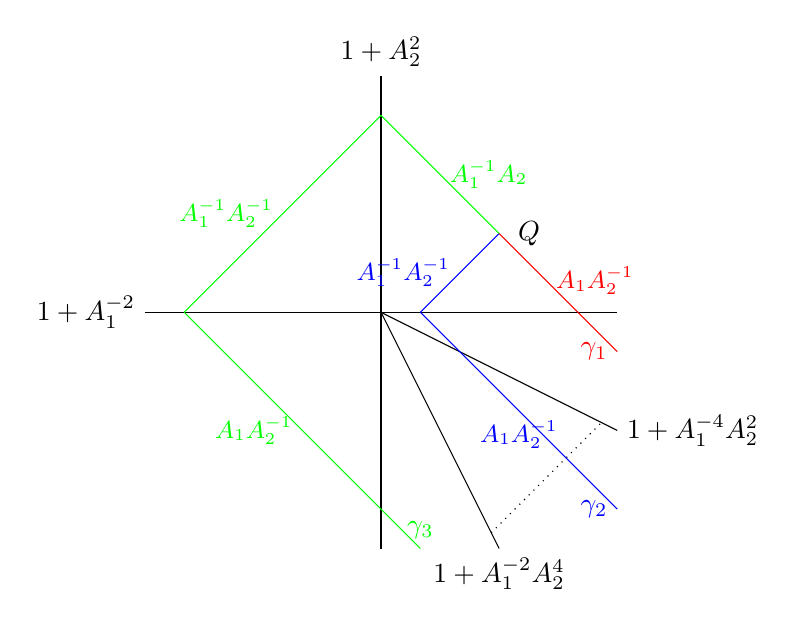
\begin{tikzpicture}
    \draw (3,0) -- (-3,0) node[left] {$1+A_1^{-2}$};
    \draw (0,-3) -- (0,3) node[above] {$1+A_2^2$};
    \draw (0,0) -- (3,-1.5) node[right] {$1+A_1^{-4}A_2^2$};
    \draw (0,0) -- (1.5,-3) node[below] {$1+A_1^{-2}A_2^4$};
    \draw (1.5,1) node[circle, right] {$Q$};
    \draw[dotted] (1.4,-2.8) -- (2.8,-1.4);
    \draw[red] (3,-0.5) -- (1.5,1);
    \draw[red] (2.1,0.1) node[above right]{\small $A_1 A_2^{-1}$};
    \draw[red] (3,-0.5) node[left]{$\gamma_1$};
    \draw[blue] (0.5,0) -- node[left] {\small $A_1^{-1} A_2^{-1}$}  (1.5,1);
    \draw[blue] (0.5,0) -- node[below] {\small $A_1 A_2^{-1}$} (3,-2.5);
    \draw[blue] (3,-2.5) node[left]{$\gamma_2$};
    \draw[green] (0,2.5)  -- node[right] {\small $A_1^{-1}A_2$} (1.5,1);
    \draw[green] (-2.5,0) -- node[left] {\small $A_1^{-1} A_2^{-1}$}  (0,2.5);
    \draw[green] (0.5, -3)  --node[left] {\small $A_1 A_2^{-1}$} (-2.5,0);
    \draw[green] (0.5,-3) node[above]{$\gamma_3$};
  \end{tikzpicture}
  \caption{Example~\ref{brokenex}} 
  \label{figbrokenex}
\end{figure}

The following summarizes the main properties of the theta functions as shown in
\cite{GHKK}:
\begin{theorem} $ $
  \begin{enumerate}
    \item
      If $\DD$ is any consistent scattering diagram, $Q$, $Q'$ are two general
      irrational points on $M_{\RR} \backslash$ Supp$(\DD)$, and $\gamma$ is a
      path joining $Q$ to $Q'$, then 
      \[
        \theta_{\gamma, \DD }(\vartheta_{Q,m}) = \vartheta_{Q', m}. 
      \]
    
    \item 
      Taking $\DD=\DD_{(b,c)}$, if $Q$ lies in the interior of a chamber of
      $\DD$, then $\vartheta_{Q,m}$ is a Laurent polynomial for any $m$.
    
    \item 
      Taking $\DD=\DD_{(b,c)}$, if $Q$ lies in the interior of the first
      quadrant, then $\vartheta_{Q,m}$ is a universal Laurent polynomial for
      any $m$.

    \item 
      Taking $\DD=\DD_{(b,c)}$, if $m$ lies in the interior of a chamber of
      $\DD$, and $Q$ lies in the same chamber, then $\vartheta_{Q,m}=z^{m}$.
   
  \end{enumerate}
\end{theorem}

\begin{proof}
  (1) is a main result of \cite{CPS}, quoted in this context in \cite{GHKK},
  Theorem 3.5.  The second statement is \cite{GHKK}, Example 7.18: there,
  $\Theta$ is the subset of $M$ consisting of those $m$ for which
  $\vartheta_{Q,m}$ is a Laurent polynomial for $Q$ in the interior of 
  some chamber of $\DD$ (and hence by \cite{GHKK}, Proposition 7.1, all 
  chambers).
  Next, (3) follows from (2) by Theorem \ref{univLaurent}. 
  Finally, (4) follows from \cite{GHKK}, Proposition 3.8 (use the argument of
  \cite{GHKK}, Theorem 4.8 in the case that the chamber is not the positive
  quadrant.)
\end{proof}

\begin{remark} 
  \label{rk:theta functions g-vector}
  If $m\in M$ lies in one of the chambers of $\DD_{(b,c)}$, and $Q$ lies in
  the first quadrant, then from (1) and (4) of the above theorem,
  $\vartheta_{Q,m}=\theta_{\gamma,\DD_{(b,c)}}(z^{m})$ for a path $\gamma$
  joining the chamber containing $m$ to $Q$. Moreover it follows from the
  details of the proof of Theorem \ref{univLaurent} that $\vartheta_{Q,m}$ is
  a cluster monomial, and from \cite{GHKK}, Theorem 7.5, that the 
  ${\bf g}$-vector of this cluster monomial is precisely $m$. 
\end{remark}

\begin{example}
  Let us try one more calculation with broken lines. We take the same scattering
  diagram as in example~\ref{brokenex}. Now take the initial slope $m=2(f_1-f_2)$
  with the same endpoint $Q$. By similar calculations we get 
  \[ 
    \vartheta _{Q, 2(f_1-f_2)} = 
    A_1^2 A_2^{-2} + A_1^{-2}A_2^2 + A_1^{-2}A_2^{-2} + 2 A_2^{-2} + 2A_1^{-2}.  
  \]
  Note that 
  \[ 
    \vartheta _{Q, 2(f_1-f_2)} = 
    (\vartheta_{Q,f_1-f_2}) ^2 -2. 
  \]
  In this scattering diagram $\DD_{(2,2)}$, the ray with slope $f_1-f_2$ does
  not lie in the interior of any chamber. So neither $\vartheta_{Q,f_1-f_2}$ nor 
  $\vartheta _{Q, 2(f_1-f_2)}$ are cluster monomials.

  There are a number of known bases for $\cA(2,2)$, which give different results
  for the basis elements with ${\bf g}$-vectors $(d,-d)$ for $d>0$. Our
  calculations shows that at least for $d=1$ or $2$, theta functions agree with
  the greedy basis elements.
\end{example}


\section{Relation to greedy bases}
\saySS{At a certain point in our discussion in Snowbird we decided we were going
  to use the scattering diagram $\DD_{\mathrm{gr},(b,c)}$ instead of
  $-\DD_{\mathrm{gr},(b,c)}$ because we would have the base point $Q$ in the
  first quadrant and most of the rays in the third one. By doing so we get that
  theta functions in $\DD_{\mathrm{gr},(b,c)}$ are parametrized by the
  \emph{negative} of their ${\bf d}$-vectors. On the other hand, in
  $\DD_{(b,c)}$ theta functions are parametrized by their ${\bf g}$-vectors.
  This is slightly counterintuitive, maybe it is  more natural to change
  our convention.}
\sayMG{I would be slightly inclined to stick with the convention we
  are currently using in the paper, as it is a less drastic change
  from what is used in GHKK}
As mentioned in Remark \ref{rk:theta functions g-vector}, theta functions are
parametrized by their ${\bf g}$-vectors. On the other hand the description of
greedy elements given in \cite{LLZ} is in terms of their ${\bf d}$-vectors (cf.
Remark 1.9 ibid.). 

In order to compare the two we will leverage the observation that, in rank 2,
these families of vectors are related by an easy piecewise-linear transformation
as explained in the paragraph following Conjecture 3.21 in \cite{RS}. We will do
so via a scattering diagram $\DD_{\mathrm{gr},(b,c)}$ closely related to
$\DD_{(b,c)}$.

Let $e_1,e_2$ be the dual basis of $f_1, f_2$, and define a piecewise-linear map
$T:M_\RR\rightarrow M_\RR$ given by
\[
  T (m) := 
  \begin{cases}
    m   & \langle e_2 , m \rangle \geq 0 \\
    m + b f_1 \langle e_2, m \rangle & \langle e_2, m \rangle \leq 0.
  \end{cases}
\]
We will denote its domains of linearity by 
\[ 
  \mathcal{H}_{+} := 
  \{ m \in M_{\mathbb{R}}\, |\, \langle e_2 , m \rangle \geq 0 \} 
  \quad
  \mbox{and}
  \quad
  \mathcal{H}_{-} := 
  \{ m \in M_{\mathbb{R}} \,|\, \langle e_2 , m \rangle \leq 0 \}.
\]
Let $T_+$ and $T_-$ be the linear extensions to $M_\RR$ of $T|_{\mathcal{H}_+}$
and $T|_{\mathcal{H}_-}$ respectively ($T_+$ is just the identity map but it
will be convenient to use this notation in what follows). 
By (\ref{eqn:linear action}) both $T_+$ and $T_-$ act on pairs $(\dd,f_\dd)$ so
we can use them to define the image of such pairs under $T$. Namely set
\[
  T(\dd,f_\dd):=
  \left\{
    T_+\left(\dd\cap\mathcal{H}_+,f_\dd\right),
    T_-\left(\dd\cap\mathcal{H}_-,f_\dd\right)
  \right\}.
\]

Having fixed the notation we are ready to introduce $\DD_{\mathrm{gr},(b,c)}$.
The set
\[
  T(\DD_{(b,c)}):=
  \left\{
    T(\dd,f_\dd)\, |\, (\dd,f_\dd)\in \DD_{(b,c)}
  \right\}
\]
is not a scattering diagram according to Definition 
\ref{def:scattering_diagram} (not all of its elements are walls for the same
convex cone) but can be made into one by few quick fixes.

First of all $\big( \RR f_2, 1+A_2^c\big)$ is the only wall of $\DD_{(b,c)}$
whose support is not totally contained in one of the domains of linearity of
$T$; therefore, under $T$, it breaks into two parts:
\[
  \big( \RR_{\ge0} f_2, 1+A_2^c\big)
  \quad
  \mbox{and}
  \quad
  \big( \RR_{\le 0} (bf_1+f_2), 1+A_1^{bc}A_2^c\big).
\]

Next note that, since $T(-f_1)=-f_1$ and $T(bf_1-f_2)=-f_2$, $T$ maps all the
walls of $\DD_{(b,c)}\setminus\DD_{\mathrm{in},(b,c)}$ to the third quadrant. 
Indeed $\big(\RR_{\leq0}(-bf_1+f_2),1+A_1^{-bc}A_2^c\big)$ is the wall with the
biggest slope in $\DD_{(b,c)}\setminus\DD_{\mathrm{in},(b,c)}$; its image is
$\big( \RR_{\le0} f_2, 1+A_2^c\big)$.

\begin{defn}
  $\DD_{\gr,(b,c)}$ is the scattering diagram obtained from
  $T(\DD_{(b,c)})$ by replacing 
  \begin{itemize}
    \item
      $\big(\RR (-f_1), 1+A_1^{-b}\big)$ with $\big(\RR  f_1, 1+A_1^b\big)$,
    
    \item 
      both $ \big( \RR_{\ge0} f_2, 1+A_2^c\big)$ and $\big( \RR_{\le0} f_2,
      1+A_2^c\big)$ with $ \big( \RR f_2, 1+A_2^c\big)$.
  \end{itemize}
  Its base region is the cone $\sigma_\gr$ generated by $f_1$ and $f_2$.
\end{defn}

\begin{remark}
  It is not too hard to see that the scattering diagram $\DD_{\gr,(b,c)}$ is
  consistent. This fact, together with the uniqueness property implied by
  \cite[Theorem 1.7]{GHKK}, gives an alternative way to introduce it. Indeed, in
  analogy with the definition of $\DD_{(b,c)}$, one could consider the
  scattering diagram
  $\DD_{\gr,\mathrm{in},(b,c)}$ given by
  \[
    \DD_{\gr,\mathrm{in},(b,c)}=
    \left\{
      \big(\RR f_1, 1+A_1^b\big), 
      \big(\RR f_2, 1+A_2^c\big)
    \right\}
  \]
  and obtain $\DD_{\gr,(b,c)}$ using Theorem \ref{KS}. 
\end{remark}

For a broken line $\gamma$ in $\DD_{(b,c)}$, we denote its image under $T$ as
$T(\gamma)$: this is the broken line in $\DD_{\gr,(b,c)}$ whose underlying map
is $\gamma\circ T$. Given any domain of linearity $L$ of $\gamma$, by
subdividing it when necessary, we can always assume that either $\gamma(L)
\subset \mathcal{H}_{+} $ or $\gamma(L)\subset \mathcal{H}_{-}$. The monomial
attached to $L$ in $T(\gamma)$ is then obtained by applying, accordingly, either
$T_+$ or $T_-$ to the exponent of the monomial attached to $L$ in $\gamma$.

\begin{theorem}
  \label{thm:T_on_broken_lines}
  $T$ defines a one-to-one correspondence between broken lines in $\DD_{(b,c)}$
  for $m$ with endpoint $Q$ and broken lines in $\DD_{\gr,(b,c)}$ for $T(m)$
  with endpoint $T(Q)$. In particular for $Q \in \mathcal{H}_+$ or $\mathcal{H}_-$,
  we have
  \[ 
    \vartheta^{\gr}_{T(Q),T( m)} = 
    T_{+} (\vartheta_{Q, m}) 
    \quad
    \mbox{or} 
    \quad
    T_{-} (\vartheta_{Q, m})
  \]
  respectively.
\end{theorem}

\begin{proof}
  This is essentially the same as the argument of \cite{GHKK}, Prop.\ 3.6.  To
  prove the statement, we only need to check the bending at the $x$-axis. Let
  $L_1$, $L_2$ be the domains of linearity of $\gamma$ before and after bending
  along $\RR (-f_1)$. So $c_{L_2} z^{m_{L_2}}$ is a term in 
  \[
    \theta_{-m_{L_1},\RR(-f_1)} (c_{L_1} z^{m_{L_1}})
    = 
    c_{L_1} z^{m_{L_1}} (1+A_1^{-b}) ^{|\langle  m_{L_1}, e_2  \rangle|}.
  \]

  First, assume $\gamma$ passes from $\mathcal{H}_-$ to $\mathcal{H}_+$. In this
  case, we have $\langle m_{L_1}, e_2 \rangle < 0$. Now in order for the monomial
  $c_{L_2}z^{T_+(m_{L_2})} =c_{L_2}z^{m_{L_2}}$ attached to $L_2$ in
  $T\circ\gamma$ to satisfy the bending rule, it must be a term in
  \[
    \theta_{-T_-(m_{L_1}),\RR f_1} (c_{L_1} z^{T_-(m_{L_1})}). 
  \]
  Since 
  \[
    \langle T_-(m_{L_1}), e_2\rangle 
    =
    \langle m_{L_1}+bf_1\langle e_2, m_{L_1} \rangle, e_2\rangle
    =
    \langle m_{L_1}, e_2 \rangle
  \]
  we get
  \begin{align*} 
    \theta_{-T_-(m_{L_1}),\RR f_1} (c_{L_1} z^{T_-(m_{L_1})}) 
    & =
    c_{L_1} z^{T_-(m_{L_1})} (1+A_1^b) ^{-\langle T_-(m_{L_1}), e_2\rangle}
    \\
    & = 
    c_{L_1} z^{m_{L_1}} A_1^{b\langle m_{L_1}, e_2\rangle} 
    (1+A_1^b)^{- \langle m_{L_1}, e_2 \rangle} 
    \\
    & = 
    c_{L_1} z^{m_{L_1}} (1+A_1^{-b}) ^{-\langle  m_{L_1}, e_1  \rangle}.
  \end{align*}
  This shows that $T_k(\gamma)$ satisfies the correct rule when bending along
  $(\RR f_1, 1+A_1^b)$ if $\gamma$ passes from $\mathcal{H}_-$ to
  $\mathcal{H}_+$. By repeating similar calculations, we can see that this also
  holds when $\gamma$ passes from $\mathcal{H}_+$ to $\mathcal{H}_-$.
\end{proof}

The following demonstrates the utility of using $\DD_{\gr,(b,c)}$:

\begin{prop}
  For any  $m\in M$, if $Q$ lies in the first quadrant, then 
  \[
    \vartheta^{\gr}_{Q, m}=z^{m}(1+f(A_1,A_2))
  \]
  where $f\in (A_1,A_2)\subseteq \Bbbk[A_1,A_2]$.
  In particular, $m$ is the negative of the ${\bf d}$-vector of
  $\vartheta^{\gr}_{Q,m}$.
\end{prop}

\begin{proof}
  For any $m\in M$ and any $Q$ in the first quadrant, there is always a broken
  line $\gamma$ for $m$ and $Q$ that does not bend at any wall. Therefore $\Mono
  (\gamma) = z^{m}$ always appears as a term in $\vartheta^{\gr}_{Q,m}$.

  However, because the functions attached to the walls of
  $\DD_{\gr,(b,c)}$ are all of the form $1+g(A_1,A_2)$ with $g(A_1,A_2) \in
  (A_1,A_2) \subseteq \Bbbk[[A_1,A_2]]$, it follows that any term coming from a
  broken line which bends must be of the form $cz^{m}A_1^{d_1}A_2^{d_2}$ with
  $d_1,d_2\ge 0$, $d_1+d_2>0$. This proves the result.
\end{proof}

\sayMG{It might be appropriate to add stuff about the quantum version here.
  Right now I don't know if we can easily prove enough facts about the quantum
  version for our main result. I suggest we wait until the rest is written up
  and then I see whether it is possible to extend the proof given what we
  currently know. (For example, in general I don't know how to get the chamber
  structure that is visible in the classical case.)}

\begin{remark}
  Combining Theorem \ref{thm:T_on_broken_lines} with the above result, when $Q$
  is in the first quadrant we obtain the parametrization of
  theta functions we were after. Indeed we get 
  \[
    \vartheta^\gr_{Q,T(m)}=\vartheta_{Q,m}
  \]
  with $m$ being its ${\bf g}$-vector and $T(m)$ the negative of its 
  ${\bf d}$-vector.
\end{remark}

\begin{thebibliography}{99}
  
  \bibitem[CPS]{CPS} M.~Carl, M.~Pumperla, and B.~Siebert, A tropical view of Landau-Ginzburg models, available at http://www.math.uni-hamburg.de/home/siebert/preprints/LGtrop.pdf
  \bibitem[G10]{G10} M.~Gross,  \emph{Mirror symmetry for $\mathbb{P}^2$ and tropical geometry}, Adv.\ Math., {\bf 224} (2010), 169--245. \bibitem[GHK11]{GHK11} M.~Gross, P.~Hacking and S.~Keel, \emph{Mirror symmetry for log Calabi-Yau surfaces I}, preprint, 2011.
  \bibitem[GHKK]{GHKK} M.~Gross, P.~Hacking, S.~Keel, M.~Kontsevich, \emph{Canonical bases for cluster algebras}, preprint, 2014.
  \bibitem[IOTW]{IOTW} K.~Igusa, K.~Orr, G.~Todorov, J.~Weyman \emph{Picture groups of finite type and cohomology in type $A_n$}, preprint, available at http://people.brandeis.edu/~igusa/Papers/PictureGroup.pdf 
  \bibitem[LLZ]{LLZ}K.~Lee, L.~Li, A.~Zelevinsky \emph{Greedy elements in rank 2 cluster algebras}, Selecta Math. (N.S.), {\bf 20}, (2014), 57--82,
  \bibitem[R]{R} N.~Reading, \emph{Universal geometric cluster algebras}, Mathematische Zeitschrift, {\bf 277 } (2014), 499-547.
  \bibitem[RS]{RS} N.~Reading, D.~Speyer, \emph{Combinatorial frameworks for cluster algebras}, preprint, 2011.

\end{thebibliography}

\end{document}
